%! TeX program = lualatex
\documentclass[tikz, crop]{standalone}
\usepackage{amssymb}

\input{../typography.tex.preamble}
\input{../tikz.tex.preamble}

\pgfplotsset{
  derivative test intro/.style = {
    basic curve,
    width={150pt},
    enlargelimits,
    axis lines=box,
    xtick={\empty}, ytick={\empty},
    xlabel={\empty}, ylabel={\empty},
    gray!50,
  }
}


\pgfplotsset{
  derivative test/.style = {
    ymin=-8, ymax=2,
    xmin=-5, xmax=6,
    xticklabel={\empty},
    yticklabel={\empty},
    width={200pt},
  }
}
\begin{document}
\begin{tikzpicture}
  \begin{axis}[derivative test intro]
    \addplot[black, very thick, domain=-0.9:0] {sqrt(1-x^2)};
  \end{axis}
\end{tikzpicture}

\begin{tikzpicture}
  \begin{axis}[derivative test intro]
    \addplot[black, very thick, domain=0:0.9] {-sqrt(1-x^2)};
  \end{axis}
\end{tikzpicture}

\begin{tikzpicture}
  \begin{axis}[derivative test intro]
    \addplot[black, very thick, domain=0:0.9] {sqrt(1-x^2)};
  \end{axis}
\end{tikzpicture}

\begin{tikzpicture}
  \begin{axis}[derivative test intro]
    \addplot[black, very thick, domain=-0.9:0] {-sqrt(1-x^2)};
  \end{axis}
\end{tikzpicture}

\begin{tikzpicture}
  \begin{axis}[
    basic curve,
    enlargelimits={0.05},
    axis equal image=false,
    xtick={-3*pi/2, -pi, -pi/2, 0, pi/2, pi, 3*pi/2},
    xticklabels={},
    ytick={-1,1},
    xlabel={\empty}, 
    ylabel={\empty},
    ]
    \addplot[very thick, domain=-3*pi/2:0] {sin(x) + x/2/pi};
    \addplot[very thick, domain=0:pi/2] {0};
    \addplot[very thick, domain=pi/2:3*pi/2] {sin(x-pi/2) + (x-pi/2)/2/pi};
    \node at (axis cs:pi/2,1) {\(f'(x)\)};
  \end{axis}
\end{tikzpicture}

% sage: f(x) = ((x+1)*(x-2)).integrate(x).integrate(x)
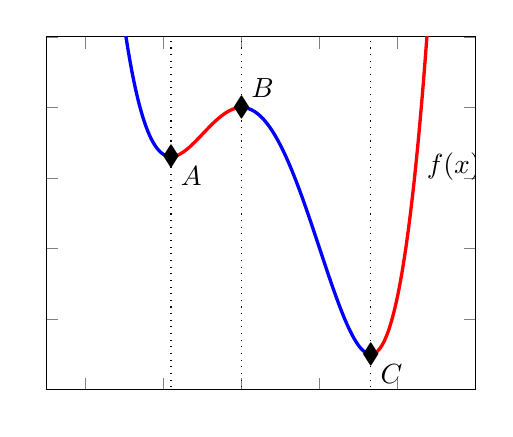
\begin{tikzpicture}
  \begin{axis}[derivative test]
    \addplot[very thick, smooth, domain=-4:-1.81174, blue] {1/12*x^4 - 1/6*x^3 - x^2};
    \addplot[very thick, smooth, domain=-1.81174:0, red] {1/12*x^4 - 1/6*x^3 - x^2};
    \addplot[very thick, smooth, domain=0:3.31174, blue] {1/12*x^4 - 1/6*x^3 - x^2};
    \addplot[very thick, smooth, domain=3.31174:6, red] {1/12*x^4 - 1/6*x^3 - x^2};
    \node at (-1.81174,-1.39341) {\(\blacklozenge\)};
    \node[below right] at (-1.81174,-1.39341) {\(A\)};
    \node at (0.00000,0.00000) {\(\blacklozenge\)};
    \node[above right] at (0.00000,0.00000) {\(B\)};
    \node at (3.31174,-6.99721) {\(\blacklozenge\)};
    \node[below right] at (3.31174,-6.99721) {\(C\)};

    \addplot[dotted, thin] coordinates { (-1.81174, -10) (-1.81174, 10) };
    \addplot[dotted, thin] coordinates { (0, -10) (0, 10) };
    \addplot[dotted, thin] coordinates { (3.31174, -10) (3.31174, 10) };

    \node[below right] at (4.5,-1) {\(f(x)\)};
  \end{axis}
\end{tikzpicture}

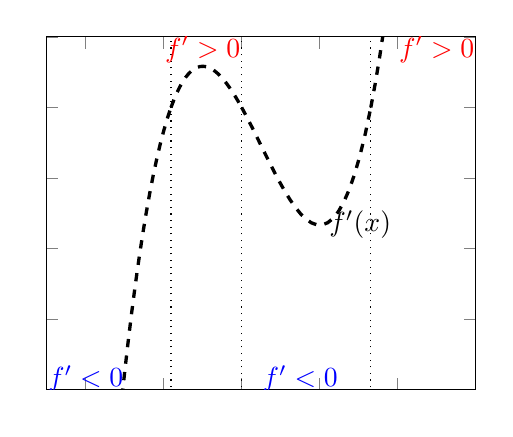
\begin{tikzpicture}
  \begin{axis}[derivative test]

    \addplot[dashed, very thick, domain=-4:-1.81174] {1/3*x^3 - 1/2*x^2 - 2*x};
    \addplot[dashed, very thick, domain=-1.81174:0] {1/3*x^3 - 1/2*x^2 - 2*x};
    \addplot[dashed, very thick, domain=0:3.31174] {1/3*x^3 - 1/2*x^2 - 2*x};
    \addplot[dashed, very thick, domain=3.31174:6] {1/3*x^3 - 1/2*x^2 - 2*x};

    \addplot[dotted, thin] coordinates { (-1.81174, -10) (-1.81174, 10) };
    \addplot[dotted, thin] coordinates { (0, -10) (0, 10) };
    \addplot[dotted, thin] coordinates { (3.31174, -10) (3.31174, 10) };

    \node[above right] at (2, -4) {\(f'(x)\)};

    \node[blue] at (-4, -7.7) {\(f'<0\)};
    \node[red, above] at (-1, 1) {\(f'>0\)};
    \node[blue] at (1.5, -7.7) {\(f'<0\)};
    \node[red, above] at (5, 1) {\(f'>0\)};
  \end{axis}
\end{tikzpicture}

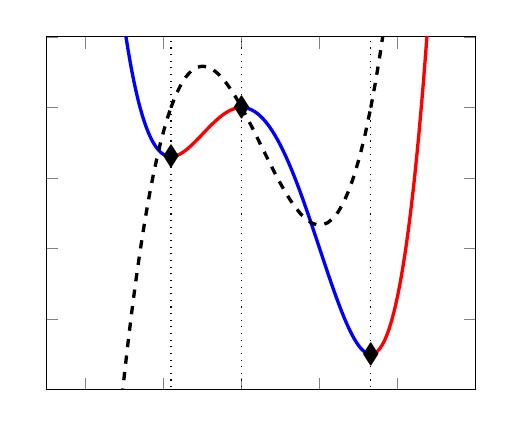
\begin{tikzpicture}
  \begin{axis}[derivative test]
    \addplot[very thick, smooth, domain=-4:-1.81174, blue] {1/12*x^4 - 1/6*x^3 - x^2};
    \addplot[very thick, smooth, domain=-1.81174:0, red] {1/12*x^4 - 1/6*x^3 - x^2};
    \addplot[very thick, smooth, domain=0:3.31174, blue] {1/12*x^4 - 1/6*x^3 - x^2};
    \addplot[very thick, smooth, domain=3.31174:6, red] {1/12*x^4 - 1/6*x^3 - x^2};
    \node at (-1.81174,-1.39341) {\(\blacklozenge\)};
    \node at (0.00000,0.00000) {\(\blacklozenge\)};
    \node at (3.31174,-6.99721) {\(\blacklozenge\)};

    \addplot[dotted, thin] coordinates { (-1.81174, -10) (-1.81174, 10) };
    \addplot[dotted, thin] coordinates { (0, -10) (0, 10) };
    \addplot[dotted, thin] coordinates { (3.31174, -10) (3.31174, 10) };

    \addplot[dashed, very thick, domain=-4:-1.81174] {1/3*x^3 - 1/2*x^2 - 2*x};
    \addplot[dashed, very thick, domain=-1.81174:0] {1/3*x^3 - 1/2*x^2 - 2*x};
    \addplot[dashed, very thick, domain=0:3.31174] {1/3*x^3 - 1/2*x^2 - 2*x};
    \addplot[dashed, very thick, domain=3.31174:6] {1/3*x^3 - 1/2*x^2 - 2*x};

    \addplot[dotted, thin] coordinates { (-1.81174, -10) (-1.81174, 10) };
    \addplot[dotted, thin] coordinates { (0, -10) (0, 10) };
    \addplot[dotted, thin] coordinates { (3.31174, -10) (3.31174, 10) };
  \end{axis}
\end{tikzpicture}

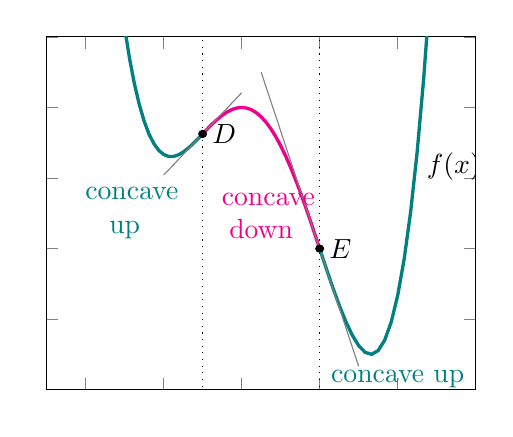
\begin{tikzpicture}
  \begin{axis}[derivative test]
    \addplot[very thick, teal, domain=-4:-1] {1/12*x^4 - 1/6*x^3 - x^2};
    \addplot[very thick, magenta, domain=-1:2] {1/12*x^4 - 1/6*x^3 - x^2};
    \addplot[very thick, teal, domain=2:6] {1/12*x^4 - 1/6*x^3 - x^2};
    \addplot[thin, gray, domain=0.5:3] {8/3 - 10*x/3};
    \addplot[thin, gray, domain=-2:0] {7*x/6 + 5/12};
    \filldraw (-1,-3/4) circle (0.1) node[right] {\(D\)};
    \filldraw (2,-4) circle (0.1) node[right] {\(E\)};
    \addplot[thin, dotted] coordinates { (-1, 10) (-1, -10) };
    \addplot[thin, dotted] coordinates { (2, 10) (2, -10) };
    \node[teal] at (-3, -3) {\parbox{1cm}{\centering concave\\up}};
    \node[magenta, above] at (0.5, -4) {\parbox{1cm}{\centering concave\\down}};
    \node[teal] at (4, -7.7) {concave up};

    \node[below right] at (4.5,-1) {\(f(x)\)};
  \end{axis}
\end{tikzpicture}

\begin{tikzpicture}
  \begin{axis}[derivative test]
    \addplot[thin, dotted] coordinates { (-1, 10) (-1, -10) };
    \addplot[thin, dotted] coordinates { (2, 10) (2, -10) };

    \addplot[very thick, loosely dashed, domain=-4:-1] {(x+1)*(x-2)};
    \addplot[very thick, loosely dashed, domain=-1:2] {(x+1)*(x-2)};
    \addplot[very thick, loosely dashed, domain=2:6] {(x+1)*(x-2)};

    \node[above right] at (0.5,-3) {\(f''(x)\)};

    \node[teal] at (-2.5, 1) {\(f''>0\)};
    \node[magenta] at (0.5, -7.7) {\(f''<0\)};
    \node[teal] at (4, 1) {\(f''<0\)};
  \end{axis}
\end{tikzpicture}

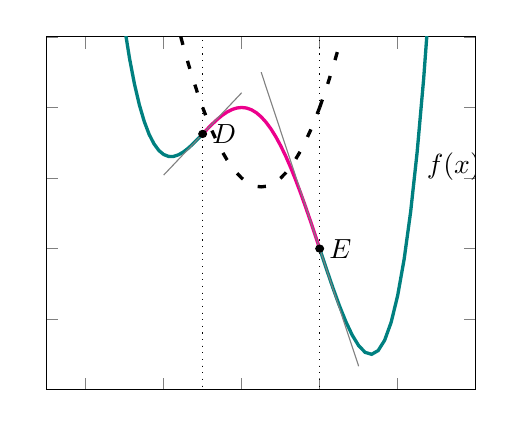
\begin{tikzpicture}
  \begin{axis}[derivative test]
    \addplot[very thick, teal, domain=-4:-1] {1/12*x^4 - 1/6*x^3 - x^2};
    \addplot[very thick, magenta, domain=-1:2] {1/12*x^4 - 1/6*x^3 - x^2};
    \addplot[very thick, teal, domain=2:6] {1/12*x^4 - 1/6*x^3 - x^2};
    \addplot[thin, gray, domain=0.5:3] {8/3 - 10*x/3};
    \addplot[thin, gray, domain=-2:0] {7*x/6 + 5/12};
    \filldraw (-1,-3/4) circle (0.1) node[right] {\(D\)};
    \filldraw (2,-4) circle (0.1) node[right] {\(E\)};
    \addplot[thin, dotted] coordinates { (-1, 10) (-1, -10) };
    \addplot[thin, dotted] coordinates { (2, 10) (2, -10) };

    \node[below right] at (4.5,-1) {\(f(x)\)};
    \addplot[thin, dotted] coordinates { (-1, 10) (-1, -10) };
    \addplot[thin, dotted] coordinates { (2, 10) (2, -10) };

    \addplot[very thick, loosely dashed, domain=-4:-1] {(x+1)*(x-2)};
    \addplot[very thick, loosely dashed, domain=-1:2] {(x+1)*(x-2)};
    \addplot[very thick, loosely dashed, domain=2:6] {(x+1)*(x-2)};
  \end{axis}
\end{tikzpicture}
\end{document}
